% !TEX root = Projektdokumentation.tex

\newglossaryentry{Usability-Tests}{name={Usability-Tests},description={Probanden aus der Zielgruppe der Anwendung werden Aufgaben gestellt, welche sie mit der bestehenden Anwendung lösen sollen. Dabei wird untersucht, welcher Weg zur Lösung der Aufgabe eingeschlagen wird und wo dabei Probleme auftauchen.}}

\newacronym{CN1}{CN1}{Computernetze 1}



%Analyse der Aufgabenstellung, Requirements Engineering, Umfeldanalyse (vergleichbare Produkte und Lösungen), Resultate der Literaturrecherche
%Auch: Ziel und Zweck von Mobile Quiz, wofür und vom wem wird es eingesetzt? Was ist zukünftiges Ziel?
%Usabilitytests, Umfeldanalyse, etc.

\section{Einleitung}
% Hier werden alle Erkenntnisse aus den einzelnen Unterkapitel zusammengefasst.
%ohne Titel

%Hier noch eine Zusammenfassung
Um ein möglichst gutes Bild davon zu erhalten, was im Bereich Online-Quizzes bereits vorhanden ist und wo dass Mobile Quiz steht, wurden Informationen von verschiedenen Bereichen gesucht und zusammengetragen.

\todo{Andrea: Zusammenfassung Recherche}

Das Testen von Mobile Quiz selbst (Punkt 8.3.1) zeigte, dass es noch einige Probleme in der Version 3 gibt. Diese zu beheben würde die Plattform solider machen und somit bestenfalls neue Quiz-Ersteller anziehen.
Weiter wurde beim Vergleich mit anderen Online-Quiz-Plattformen (Punkt 8.3.2) ersichtlich, dass Mobile Quiz im Bereich Funktionsumfang und Einstellungsmöglichkeiten gut dasteht. Problematisch wirkt sich allerdings die Usability darauf aus, denn viele Funktionen sind nur schwierig zu erreichen. Dies wurde auch durch die Usability-Tests (Abschnitt 12.1) bestätigt, welche ebenfalls zu Beginn der Arbeit durchgeführt wurden.

Die Ergebnisse aus dieser Untersuchung flossen zusammen mit den bereits bekannten Verbesserungen sowie den ToDo's von Patrick Eichler in die mögliche Aufgabenstellung dieser Studienarbeit ein. Dieses ist im Anhang unter 'MoeglicheArbeitenSA.pdf' ersichtlich. Um nicht jeden Bug einzeln aufzuführen, sondern die Probleme abstrahiert zu betrachten, wurden darin nur Themen aufgeführt und beschrieben, die verbessert werden sollten. Diese wurden dann mit dem Betreuer besprochen und priorisiert, um daraus die definitive Aufgabenstellung zu erarbeiten.

\section{Recherche/ähnliche Arbeiten}

\todo{Andrea}
%hier auch den gefundenen Standard erwähnen

\section{Eigene Untersuchungen, Webuntersuchung}

\todo{David}

Was kann Mobile Quiz heute bereits, wo gibt es noch Probleme und wo es Quiz heute im Vergleich zu ähnlichen Webanwendungen? Diese Fragen waren Kern der eigenen Untersuchungen. Einerseits wurde dazu Mobile Quiz selbst intensiv getestet, andererseits wurden mehrere vergleichbare Online-Quizzes gesucht und anhand von bestimmten Kriterien verglichen.


	\subsection{Untersuchung www.mobilequiz.ch}
	Während mehrerer Stunden wurden mit dem eigenen Benutzeraccount die vorhandenen Funktionen ausprobiert. Dabei kamen verschiedene Probleme zutage, die sich grob in die folgenden Kategorien unterteilen lassen:
	
	%Beispiele hinzufügen
	
	\begin{itemize}
		\item Sicherheitsrelevante Probleme
		\item Usability
		\item Probleme/Bugs
		\item Schreibfehler/Grammatik
		\item Allgemeine Fragen zum Konzept
		\item Mobile-Probleme
	\end{itemize}

	Die ausführlichen Resultate sind im Dokument 'Ergebnisse eigene Tests.pdf' ersichtlich.
	

	\subsection{Vergleich Online-Quizzes}
	Um andere Online-Quizzes mit Mobile Quiz zu vergleichen mussten zuerst die Kriterien festgelegt werden. Als Grundlage diente eine Excel Tabelle von Khalid Abdul und Patrik Naef, welche an die Bedürfnisse dieser Arbeit angepasst wurde.
	Die Vergleichs-Systeme wurden durch Google-Suchen und Empfehlungen von educatorstechnology.com \cite{educatorstechnology.com} ausgewählt.
	
	Die detaillierte Auswertung ist im Dokument 'SA-Mobile-Quiz\_QuizSysteme-Funktionen-Vergleich-Matrix.xlsx' ersichtlich. Nachfolgend werden wichtige Punkte daraus genauer aufgezeigt:
	
	\begin{itemize}
		\item Willkommensseite \\
		Webanwender haben eine riesige Auswahl an Seiten, welche auf ihr Bedürfnis zugeschnitten sind. Sie wenden deshalb nicht viel Zeit auf, um sich über eine einzelne Seite genauer zu informieren. Aus diesem Grund zählt oft der erste Eindruck, also eine ansprechende Willkommensseite. \\
		
		\begin{figure}[h]
			\centering
			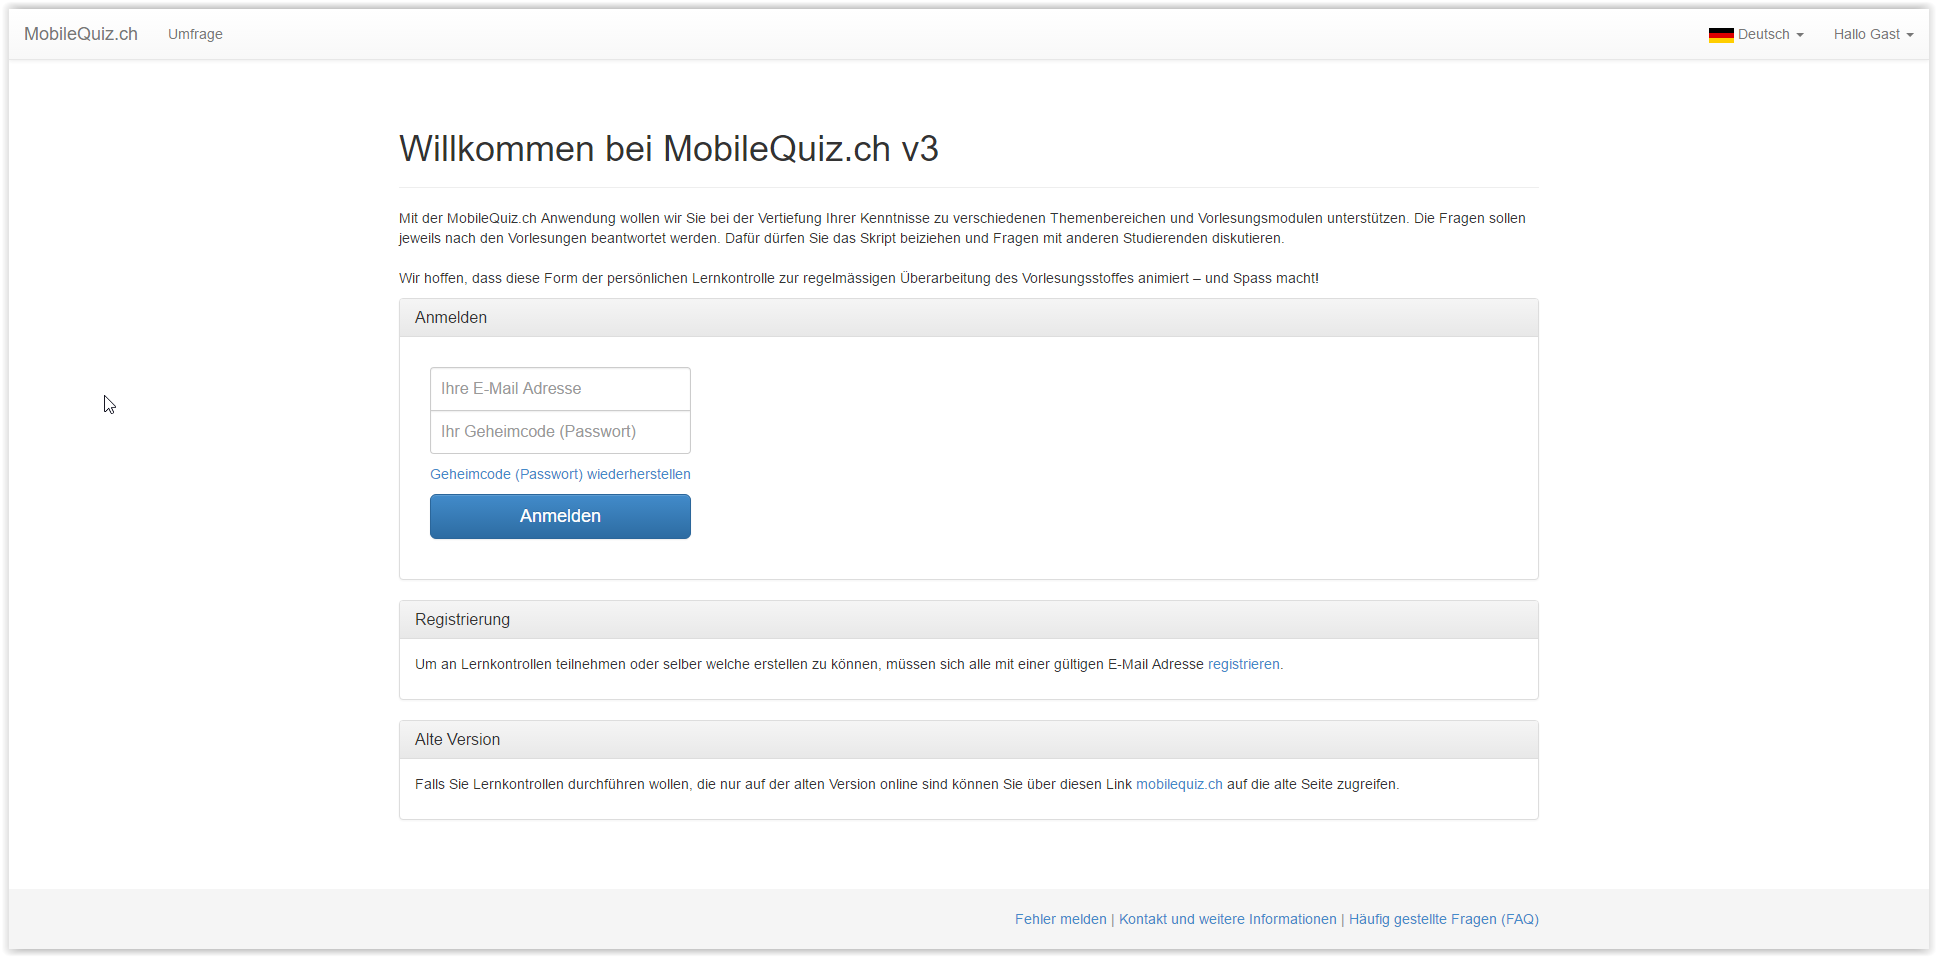
\includegraphics[width=0.5\textwidth]{Images/MobileQuiz_StartPage.PNG}
			\caption{Startseite Mobile Quiz Version 3}
		\end{figure}
		
		Ruft man www.mobilequiz.ch auf, so sieht man viel Text, der die Seite beschreibt. Ein Benutzer weiss jedoch noch nicht genau, was ihn erwartet, wenn er sich registriert und einloggt.
		
		\begin{figure}[h]
			\centering
			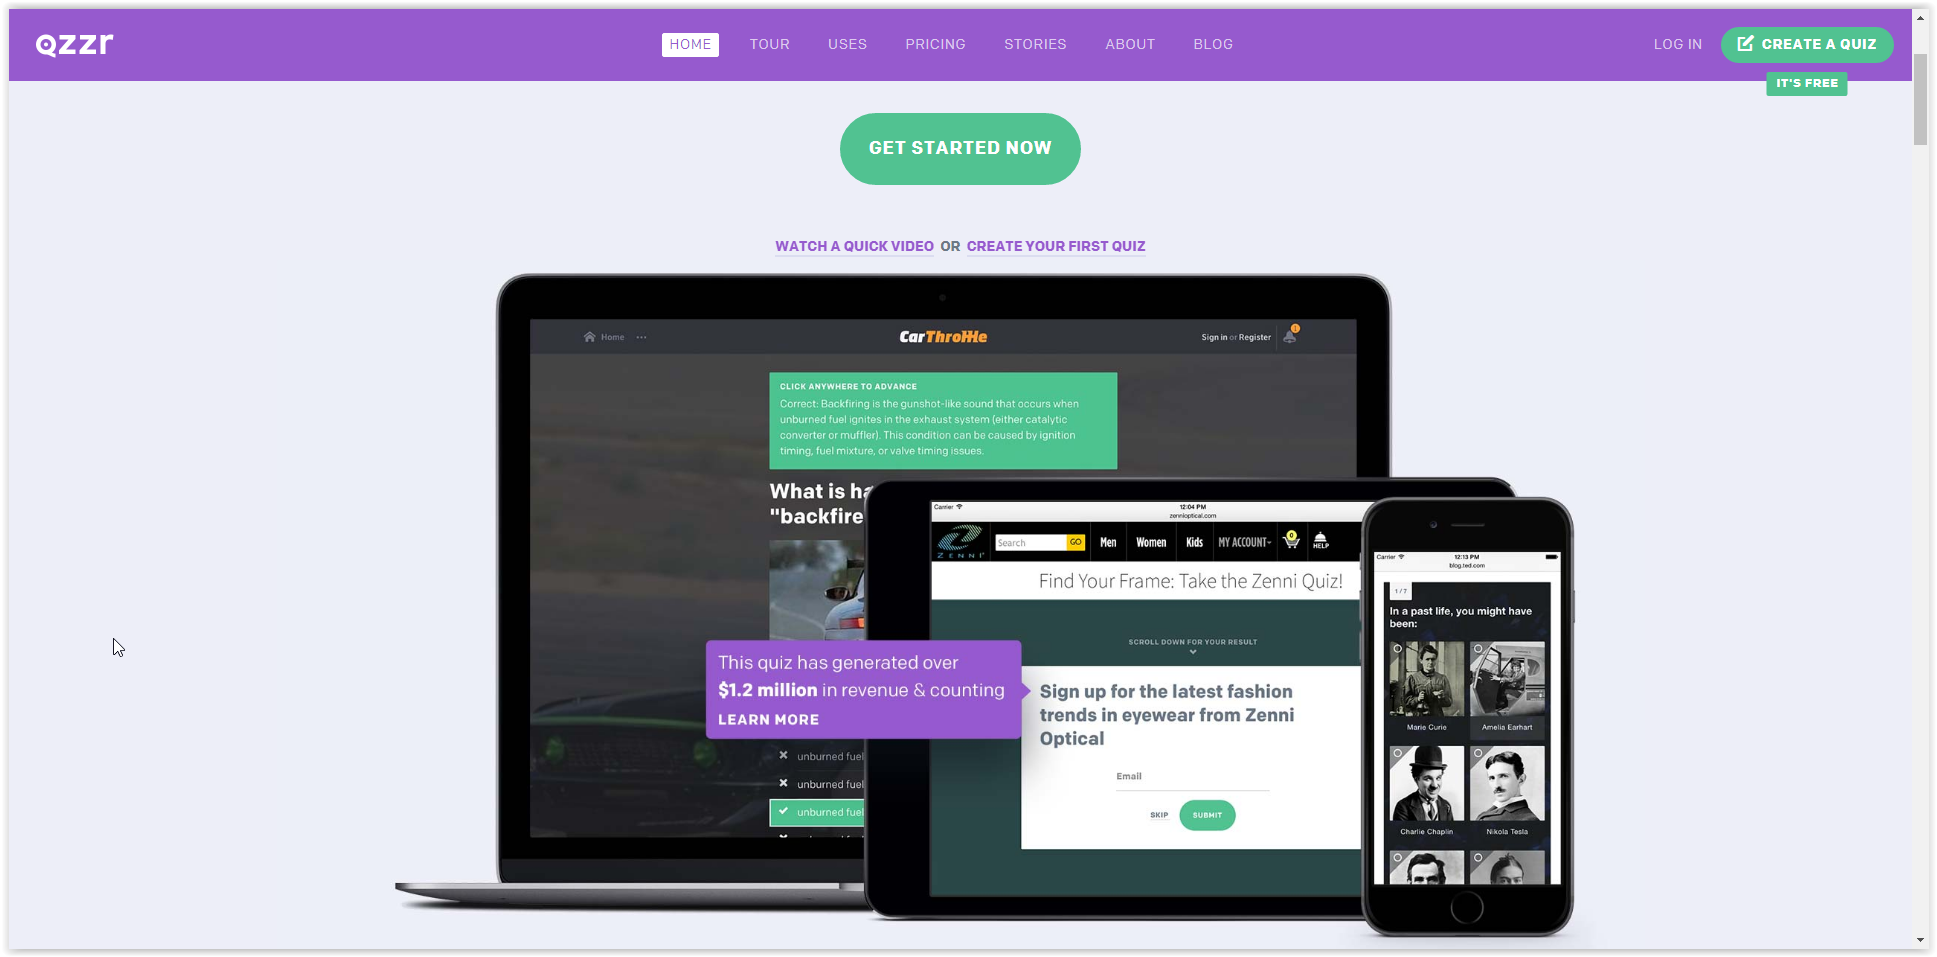
\includegraphics[width=0.5\textwidth]{Images/Qzzr_StartPage.PNG}
			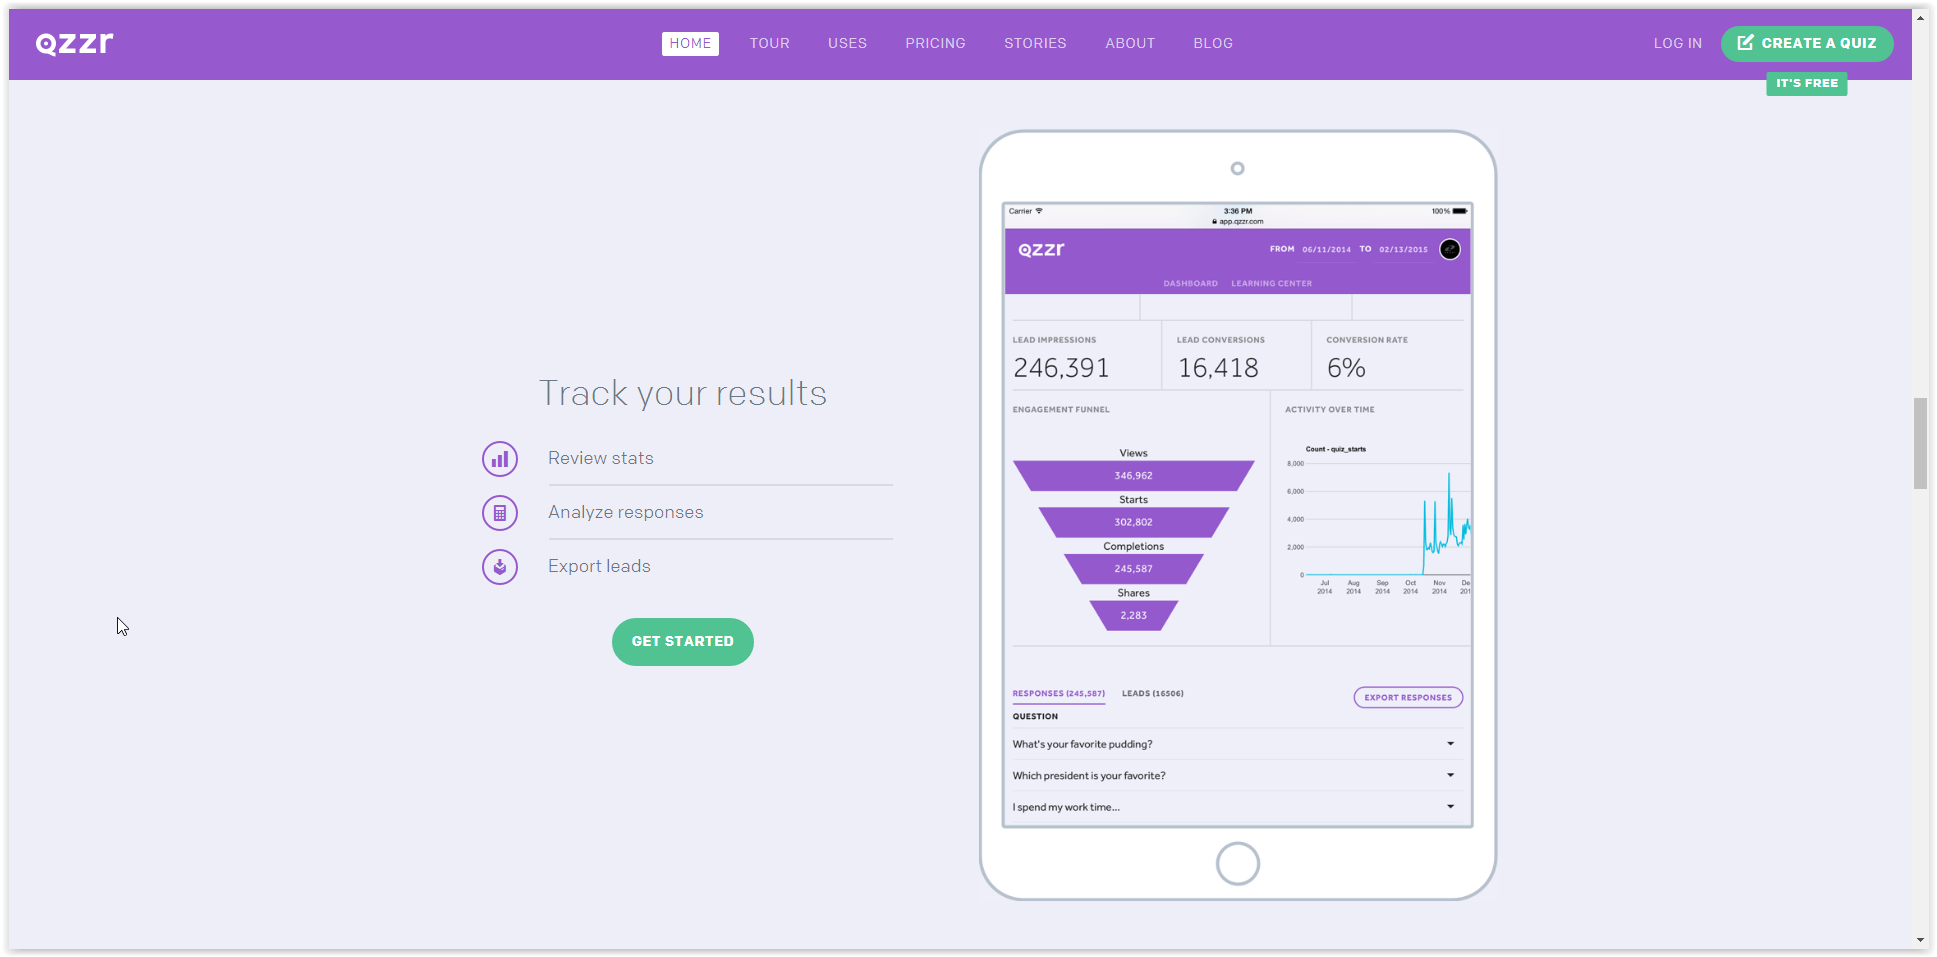
\includegraphics[width=0.5\textwidth]
			{Images/Qzzr_StartPage_Statistics.PNG}
			\caption{Startseite Qzzr}
		\end{figure}
				
		Seiten wie Qzzr \cite{qzzr.com} hingegen, zeigen anhand von Bildern und Symbolen auf, was die Funktionalitäten sind und wie diese konkret aussehen. Solche Bilder sind schnell erfasst  und verarbeitet.
		Mobile Quiz könnte die gleichen Funktionsumfang bieten, aber wenn es der Benutzer nicht sofort sieht, klickt er weiter und registriert sich andernorts.
		
		Was machen gute Willkommensseiten also aus?
		
		\todo{David: Internetrecherche}
		http://blog.hubspot.com/blog/tabid/6307/bid/34006/15-examples-of-brilliant-homepage-design.aspx
		
		
		\item Schritt für Schritt - Erstellung von Quizzes \\
		Um ein Quiz zu erstellen benötigt es einerseits die Fragen, andererseits das Quiz selbst, welches mehrere Fragen umfasst. In welcher Reihenfolge sollen diese beiden Ressourcen erstellt werden?
		Aktuell ist es bei Mobile Quiz so, dass zuerst die Fragen und anschliessend das Quiz separat erstellt wird. Ist man sich dieser Tatsache bewusst, so ist dies kein Problem, aber ist es auch intuitiv? Wie in den durchgeführten Usability-Tests festgestellt war dem nicht so. Die Benutzer, welche alle noch nie ein Quiz erstellt hatten, starteten sofort mit der Erstellung des Quizzes und mussten diese dann abbrechen.
		
		
		
		
		
		\item  Quiz-Einstellungen \\
		Quizzes können für unterschiedliche Bedürfnisse eingesetzt werden. Die möglichen Einsatzzwecke reichen von Freunden, die zum Zeitvertreib ihr Wissen gegenseitig messen wollen, über Dozenten, die prüfen möchten, ob die Studenten den Unterrichtsstoff verstanden haben, bis zu Dozenten, welche die Quizzes als Prüfung verwenden.
		Diese Situationen verlangen viele Einstellungsmöglichkeiten, welche für den Benutzer möglichst selbsterklärend sein sollen. Trifft dies jedoch nicht zu, oder ist die Darstellung unverständlich, so wird sich der Quiz-Ersteller möglicherweise nach einer anderen Quiz-Plattform umsehen.
		
		\begin{figure}[h]
			\centering
			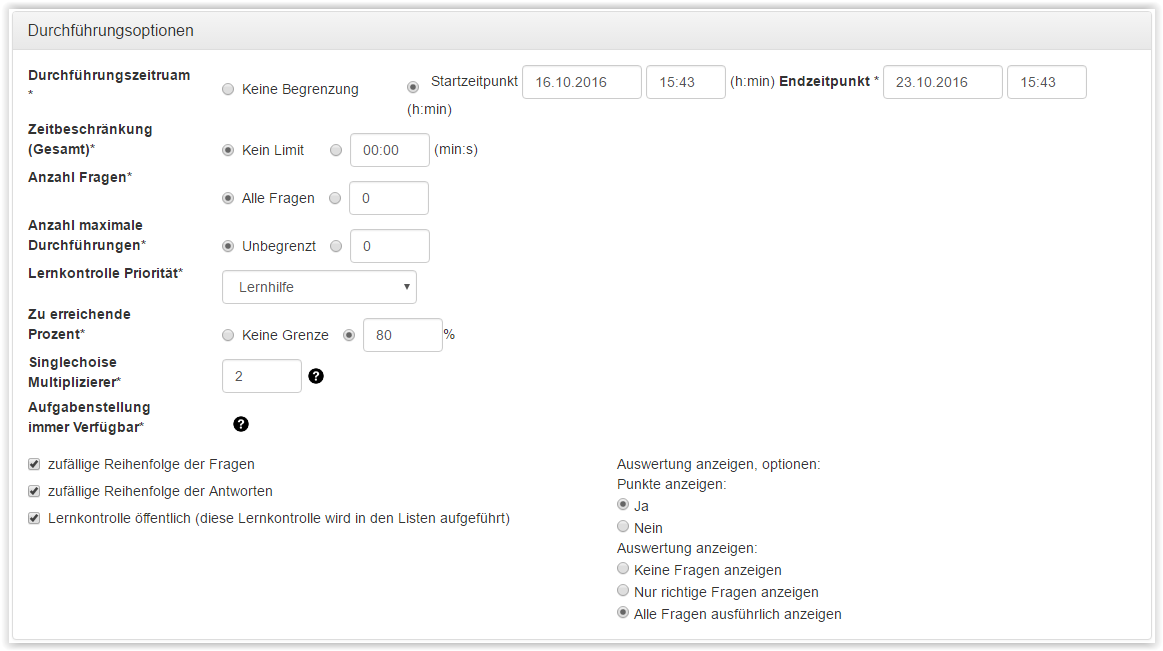
\includegraphics[width=0.5\textwidth
			]{Images/MobileQuiz_Quiz-Settings.PNG}
			\caption{Quiz-Einstellungen Mobile Quiz Version 3}
		\end{figure}
		
		
		Mobile Quiz bietet zwar derzeit viele Einstellungsmöglichkeiten an, diese sind jedoch so zahlreich, dass sie den Benutzer fast überfordern. Zudem ist die Darstellung zum Teil nicht optimal. 
		%Beispiel einfügen
		
		\begin{figure}[h]
			\centering
			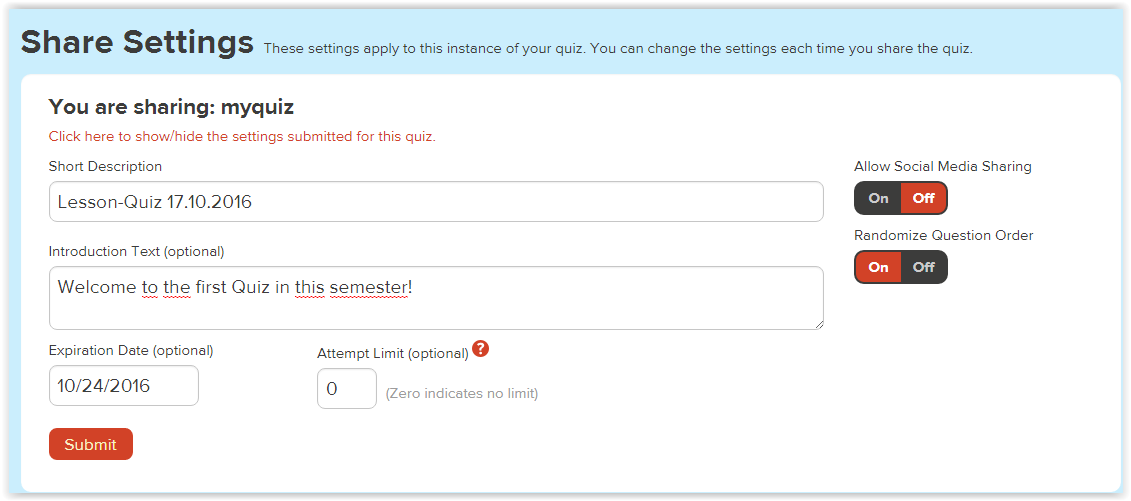
\includegraphics[width=0.5\textwidth
			]{Images/QuizBean_Quiz-Settings.PNG}
			\caption{Quiz-Einstellungen QuizBean}
		\end{figure}
		
		
		
		\item Quiz kann vor Veröffentlichung durchgespielt werden \\
		Wie sieht das erstellte Quiz für den Teilnehmer aus? Gibt es noch Rechtschreibfehler oder werden Inhalte nicht optimal dargestellt? Ein Quiz-Ersteller wird sich all diese Fragen womöglich stellen und die einfache Lösung dazu ist, dass man das Quiz vor Veröffentlichung selbst durchspielt. Die eigene Teilnahme soll jedoch nicht zählen, da sie die Auswertungsstatistik verfälschen kann.
		
		Mobile Quiz bietet derzeit eine solche Funktion an, diese Funktioniert aber nur .... %Nachprüfen
		Wird dies korrigiert, so reiht sich Mobile Quiz in diesem Punkt in die vorderen Plätze ein.
		
		
		\item Template für Frage-Import \\
		Ist man im Zug unterwegs und möchte trotzdem an einem neuen Quiz arbeiten, so fehlt meist der Internetzugang. Dies kompensiert Mobile Quiz dadurch, dass Fragen aus Excel-Dateien eingelesen und erstellt werden können. Um dies zu nutzen, benötigt es jedoch eine spezielle Formatierung, was neue Benutzer abschrecken kann, die nicht nicht Zeit aufwenden wollen, um sich einzuarbeiten. \\
		Die Lösung dazu ist eine Vorlage, also ein Excel-Template. Darin kann der Benutzer schnell und einfach Fragen erfassen und muss sich nicht um das Format kümmern. Solche Templates bietet beispielsweise
		Socrative \cite{socrative.com} an. Es es im Anhang unter 'socrativeQuizTemplate.xlsx' zu finden.
		
		Im Rahmen dieser Arbeit soll ebenfalls ein solches Template erstellt werden, welches dann Quiz-Erstellern zum Download angeboten wird.
		
		
		
	\end{itemize}	
	
	
	
	
	

















